\begin{topic}{lie-algebra}{Lie algebra}
    A \textbf{Lie algebra} is is a \tref{LA:vector-space}{vector space} $\mathfrak{g}$ over a field $k$, together with an operation $\mathfrak{g} \times \mathfrak{g} \to \mathfrak{g}, (x, y) \mapsto [x, y]$ called the \textbf{Lie bracket}, satisfying
    \begin{itemize}
        \item (\textit{bilinearity}) $[ax + by, z] = a[x, z] + b[y, z]$ and $[z, ax + by] = a[z, x] + b[z, y]$ for all $x, y, z \in \mathfrak{g}$ and $a, b \in k$,
        \item (\textit{alternativity}) $[x, x] = 0$ for all $x \in \mathfrak{g}$,
        \item (\textit{Jacobi identity}) $[x, [y, z]] + [z, [x, y]] + [y, [z, x]] = 0$ for all $x, y, z \in \mathfrak{g}$.
    \end{itemize}
\end{topic}

\begin{example}{lie-algebra}
    Consider $\mathfrak{g} = \RR^3$ with bracket operation defined by the \textit{cross product} $[x, y] = x \times y$.
\end{example}

\begin{example}{lie-algebra}
    For any \tref{DG:lie-group}{Lie group} $G$, the tangent space at the identity $\mathfrak{g} = T_e G$ has a Lie algebra structure, called the \textit{Lie algebra} of $G$. Tangent vectors $v \in T_e G$ correspond one-to-one to \textit{left invariant vector fields} on $G$, i.e. vector fields $X$ satisfying $X_g = ((L_g)_* X)_e$ for all $g \in G$, where $L_g : G \to G$ denotes left multiplication by $g$. The Lie bracket on $\mathfrak{g}$ is then given by the \tref{DG:lie-bracket-vector-fields}{Lie bracket of vector fields}. Note that the Lie bracket of left-invariant vector fields is indeed also left-invariant.
\end{example}

\begin{example}{lie-algebra}
    \begin{itemize}
        \item $\mathfrak{sl}_n(k) = \{ X \in \textup{Mat}_{n \times n}(k) : \tr X = 0 \}$ is the Lie algebra associated to the \tref{LA:special-linear-group}{special linear group}.
        \item $\mathfrak{so}_n = \{ X \in \textup{Mat}_{n \times n}(\RR) : X + X^T = 0 \}$ is the Lie algebra associated to the \tref{LA:orthogonal-group}{(special) orthogonal group}.
        \item $\mathfrak{u}_n = \{ A \in \textup{Mat}_{n \times n}(\CC) : X + X^H = 0 \}$ is the Lie algebra associated to the \tref{LA:unitary-group}{special unitary group}.
        \item $\mathfrak{su}_n = \{ A \in \textup{Mat}_{n \times n}(\CC) : X + X^H = 0 \textup{ and } \tr X = 0 \}$ is the Lie algebra associated to the \tref{LA:unitary-group}{special unitary group}.
        \item $\mathfrak{sp}_{2n}(k) = \{ A \in \textup{Mat}_{2n \times 2n}(k) : \Omega X + X^T \Omega = 0 \}$ is the Lie algebra associated to the \tref{LA:symplectic-group}{symplectic group}.
    \end{itemize}
\end{example}

\begin{example}{lie-algebra}
    For any \tref{ring}{ring} $A$ over a field $k$ (in particular matrix rings), the commutator bracket $[x, y] = xy - yx$ makes $A$ into a Lie algebra.
\end{example}

\begin{example}{lie-algebra}
    Let $e_1, \ldots, e_n$ be a basis of the underlying vector space of a Lie algebra $\mathfrak{g}$. The Lie bracket can be described by coefficients $c_{ij}^\ell \in k$, called the \textbf{structure constants}, such that $[e_i, e_j] = \sum_{\ell = 1}^{n} c_{ij}^\ell e_\ell$. These coefficients satisfy the following relations:
    \begin{itemize}
        \item (\textit{alternatively}) $c_{ij}^k + c_{ji}^k = 0$,
        \item (\textit{Jacobi identity}) $\sum_{m = 1}^{n} c_{ij}^m c_{m k}^\ell + c_{j k}^m c_{m i}^\ell + c_{k i}^m c_{m j}^\ell = 0$.
    \end{itemize}
\end{example}

\begin{topic}{lie-algebra-ideal}{Lie algebra ideal}
    An \textbf{ideal} of a \tref{lie-algebra}{Lie algebra} $\mathfrak{g}$ is a subalgebra $\mathfrak{h} \subset \mathfrak{g}$ such that $[X, H] \in \mathfrak{h}$ for all $X \in \mathfrak{g}$ and $H \in \mathfrak{h}$.
\end{topic}

\begin{example}{lie-algebra-ideal}
    For any Lie algebra $\mathfrak{g}$, the \textit{commutator ideal} $[\mathfrak{g}, \mathfrak{g}]$ is an ideal of $\mathfrak{g}$, given as the set of all elements in $\mathfrak{g}$ of the form
    \[ c_1 [X_1, Y_1] + \cdots + c_m [X_m, Y_m] , \]
    for some constants $c_i$ and vectors $X_i, Y_i \in \mathfrak{g}$.
\end{example}

\begin{topic}{ado-theorem}{Ado's theorem}
    \textbf{Ado's theorem} states that any \tref{lie-algebra}{Lie algebra} over a field of characteristic zero is isomorphic to a subalgebra of $\mathfrak{gl}_n(k)$, the Lie algebra of square matrices with the commutator bracket.
\end{topic}

\begin{topic}{nilpotent-lie-algebra}{nilpotent Lie algebra}
    A \tref{lie-algebra}{Lie algebra} $\mathfrak{g}$ is called \textbf{nilpotent} if its lower central series
    \[ \mathfrak{g} \supset [\mathfrak{g}, \mathfrak{g}] \supset [\mathfrak{g}, [\mathfrak{g}, \mathfrak{g}]] \supset [\mathfrak{g}, [\mathfrak{g}, [\mathfrak{g}, \mathfrak{g}]]] \supset \cdots \]
    terminates in the zero algebra.
\end{topic}

\begin{example}{nilpotent-lie-algebra}
    \begin{itemize}
        \item The Lie algebra given by
        \[ \mathfrak{g} = \left\{ \begin{pmatrix} 0 & x & y \\ 0 & 0 & z \\ 0 & 0 & 0 \end{pmatrix} \right\} , \]
        and the commutator bracket, is nilpotent. Namely, $[\mathfrak{g}, \mathfrak{g}]$ is the span of $\begin{pmatrix} 0 & 0 & 1 \\ 0 & 0 & 0 \\ 0 & 0 & 0 \end{pmatrix}$, and $[\mathfrak{g}, [\mathfrak{g}, \mathfrak{g}]] = \{ 0 \}$.
        
        \item The Lie algebra $\mathfrak{sl}_2(\CC)$ is not nilpotent since $[\mathfrak{sl}_2(\CC), \mathfrak{sl}_2(\CC)] = \mathfrak{sl}_2(\CC)$.
    \end{itemize}
\end{example}

\begin{topic}{solvable-lie-algebra}{solvable Lie algebra}
    A \tref{lie-algebra}{Lie algebra} $\mathfrak{g}$ is \textbf{solvable} if the \textit{derived series} of subalgebras
    \[ \mathfrak{g} = \mathfrak{g}^{(0)} \supset \mathfrak{g}^{(1)} \supset \mathfrak{g}^{(2)} \supset \cdots \]
    given by $\mathfrak{g}^{(i + 1)} = [\mathfrak{g}^{(i)}, \mathfrak{g}^{(i)}]$, results in the zero algebra. That is, $\mathfrak{g}^{(i)} = \{ 0 \}$ for some $i > 0$.
\end{topic}

\begin{example}{solvable-lie-algebra}
    Every \tref{nilpotent-lie-algebra}{nilpotent} Lie algebra is solvable, but the converse does not hold. Namely, consider the Lie algebra
    \[ \mathfrak{g} = \left\{ \begin{pmatrix} x & y \\ 0 & z \end{pmatrix} \right\} , \]
    with the commutator bracket. Then
    \[ \left[ \begin{pmatrix} x & y \\ 0 & z \end{pmatrix}, \begin{pmatrix} a & b \\ 0 & c \end{pmatrix} \right] = \begin{pmatrix} 0 & w \\ 0 & 0 \end{pmatrix} \]
    with $w = xb + yc - ya - zb$, which shows that $\mathfrak{g}^{(1)} = [\mathfrak{g}, \mathfrak{g}]$ is one-dimensional, and thus $\mathfrak{g}^{(2)} = [\mathfrak{g}^{(1)}, \mathfrak{g}^{(1)}] = \{ 0 \}$, so $\mathfrak{g}$ is solvable. However, since
    \[ \left[ \begin{pmatrix} 1 & 0 \\ 0 & -1 \end{pmatrix}, \begin{pmatrix} 0 & 1 \\ 0 & 0 \end{pmatrix} \right] = \begin{pmatrix} 0 & 2 \\ 0 & 0 \end{pmatrix} , \]
    it follows that $[\mathfrak{g}, [\mathfrak{g}, \mathfrak{g}]] = [\mathfrak{g}, \mathfrak{g}]$, so the lower central series does not terminate in the zero algebra, and thus $\mathfrak{g}$ is not nilpotent.
\end{example}

\begin{topic}{cartan-subalgebra}{Cartan subalgebra}
    A \textbf{Cartan subalgebra} of a \tref{lie-algebra}{Lie algebra} $\mathfrak{g}$ is a \tref{nilpotent-lie-algebra}{nilpotent} subalgebra $\mathfrak{h}$ whose \textit{normalizer} $N_\mathfrak{g}(\mathfrak{h}) := \{ X \in \mathfrak{g} : [X, \mathfrak{h}] \subset \mathfrak{h} \}$ equals $\mathfrak{h}$.
\end{topic}

\begin{example}{cartan-subalgebra}
    \begin{itemize}
        \item A Cartan subalgebra of $\mathfrak{gl}_n$ is the subalgebra of diagonal matrices.
        \item A Cartan subalgebra of $\mathfrak{sl}_n$ is the subalgebra of diagonal matrices with trace zero.
    \end{itemize}
\end{example}

\begin{topic}{universal-enveloping-algebra}{universal enveloping algebra}
    Let $\mathfrak{g}$ be a \tref{lie-algebra}{Lie algebra}. The \textbf{universal enveloping algebra} of $\mathfrak{g}$ is the algebra
    \[ U(\mathfrak{g}) = T(\mathfrak{g}) / I , \]
    where $T(\mathfrak{g})$ is the \tref{tensor-algebra}{tensor algebra} of $\mathfrak{g}$, and $I$ is the (two-sided) ideal generated by elements of the form $[x, y] - x \otimes y - y \otimes x$ for all $x, y \in \mathfrak{g}$.
    
    It has the universal property that for any \tref{algebra}{algebra} $A$ and Lie algebra morphism $\varphi : \mathfrak{g} \to A$, where the Lie bracket on $A$ is given by the commutator, there exists a unique algebra morphism $U(\mathfrak{g}) \to A$ such that
    \[ \begin{tikzcd} \mathfrak{g} \arrow{r} \arrow[swap]{dr}{\varphi} & U(\mathfrak{g}) \arrow[dashed]{d} \\ & A \end{tikzcd} \]
    commutes.
\end{topic}

\begin{example}{universal-enveloping-algebra}
    The Lie algebra $\mathfrak{g} = \mathfrak{sl}_2$ has a basis
    \[ H = \begin{pmatrix} 1 & 0 \\ 0 & -1 \end{pmatrix}, \quad X = \begin{pmatrix} 0 & 1 \\ 0 & 0 \end{pmatrix}, \quad Y = \begin{pmatrix} 0 & 0 \\ 1 & 0 \end{pmatrix} , \]
    satisfying the relations
    \[ [H, X] = 2X, \quad [H, Y] = -2Y, \quad [X, Y] = H . \]
    This shows that the universal enveloping algebra of $\mathfrak{sl}_2$ is given by
    \[ U(\mathfrak{sl}_2) = \CC \langle x, y, z \rangle / (zx - xz - 2x, zy - yz + 2y, xy - yz - z) . \]
\end{example}

\begin{example}{universal-enveloping-algebra}
    The universal enveloping algebra $U(\mathfrak{g})$ naturally has the structure of a \tref{hopf-algebra}{Hopf algebra}, where comultiplication, counit and the antipode are given by
    \[ \Delta(x) = x \otimes 1 + 1 \otimes x, \qquad \varepsilon(x) = 0 , \qquad S(x) = -x , \]
    for all $x \in \mathfrak{g}$. Note that $\Delta : U(\mathfrak{g}) \to U(\mathfrak{g}) \otimes U(\mathfrak{g})$ is well-defined since
    \[ \begin{aligned}
        \Delta([x, y])
            &= [x, y] \otimes 1 + 1 \otimes [x, y] \\
            &= xy \otimes 1 - yx \otimes 1 + 1 \otimes xy - 1 \otimes yx \\
            &= xy \otimes 1 - x \otimes y - y \otimes x + 1 \otimes xy - yx \otimes 1 + y \otimes x + x \otimes y - 1 \otimes yx \\
            &= (x \otimes 1 + 1 \otimes x)(y \otimes 1 + 1 \otimes y) - (y \otimes 1 + 1 \otimes y)(x \otimes 1 + 1 \otimes x) \\
            &= \Delta(x) \Delta(y) - \Delta(y) \Delta(x) \\
            &= \Delta(xy - yx)
    \end{aligned} \]
    for all $x, y \in \mathfrak{g}$.
\end{example}

\begin{topic}{poisson-algebra}{Poisson algebra}
    A \textbf{Poisson algebra} is a commutative \tref{algebra}{algebra} $A$ over a \tref{field}{field} $k$, together with an operation $\{ \cdot, \cdot \} : A \otimes_k A \to A$, called the \textbf{Poisson bracket}, making $A$ into a \tref{lie-algebra}{Lie algebra} and satisfying the \textit{Leibniz rule} $\{ f, gh \} = \{ f, g \} h + g \{ f, h \}$. % $\{ a, - \} : A \to A$ is a \tref{derivation}{$k$-derivation} for every $a \in A$.
\end{topic}

\begin{topic}{simple-lie-algebra}{(semi)simple Lie algebra}
    A \tref{lie-algebra}{Lie algebra} $\mathfrak{g}$ is \textbf{simple} if it is non-abelian and contains no non-zero proper \tref{lie-algebra-ideal}{ideals}.
\end{topic}

\begin{example}{simple-lie-algebra}
    The Lie algebra $\mathfrak{sl}_2(\CC)$ is simple. A basis for $\mathfrak{sl}_2(\CC)$is given by
    \[ H = \begin{pmatrix} 1 & 0 \\ 0 & -1 \end{pmatrix}, \quad X = \begin{pmatrix} 0 & 1 \\ 0 & 0 \end{pmatrix}, \quad Y = \begin{pmatrix} 0 & 0 \\ 1 & 0 \end{pmatrix} , \]
    satisfying the relations
    \[ [H, X] = 2X, \quad [H, Y] = -2Y, \quad [X, Y] = H . \]
    Let $\mathfrak{h}$ be a non-zero ideal of $\mathfrak{sl}_2(\CC)$. Then $\mathfrak{h}$ contains an element $Z = aX + bH + cY$ where $a, b, c \in \CC$ are not all zero. If $c \ne 0$, then $[X, [X, Z]] = -2cX$, so $X \in \mathfrak{h}$, and also $[Y, X] = -H \in \mathfrak{h}$ and hence also $[Y, H] = 2Y \in \mathfrak{h}$, which shows $\mathfrak{h} = \textup{sl}_2(\CC)$. If $c = 0$ and $b \ne 0$, then $[X, Z] = -2bX$, so $X \in \mathfrak{h}$ and similarly $\mathfrak{h} = \mathfrak{sl}_2(\CC)$. Finally, if $b = c = 0$ and $a \ne 0$, then $Z = aX$, so $X \in \mathfrak{h}$, so $h = \mathfrak{sl}_2(\CC)$.
\end{example}

\begin{topic}{semisimple-lie-algebra}{semisimple Lie algebra}
    A \tref{lie-algebra}{Lie algebra} $\mathfrak{g}$ is \textbf{semisimple} if it is the direct sum of simple Lie algebras.
\end{topic}

\begin{topic}{root-system-lie-algebra}{root system Lie algebra}
    Let $\mathfrak{g}$ be a complex \tref{semisimple-lie-algebra}{semisimple} \tref{lie-algebra}{Lie algebra}, and $\mathfrak{h}$ a \tref{cartan-subalgebra}{Cartan subalgebra}. A \textbf{root} of $\mathfrak{g}$ (relative to $\mathfrak{h}$) is an element $\alpha \in \mathfrak{h}^*$ such that
    \[ \mathfrak{g}_\alpha = \{ x \in \mathfrak{g} : [h, x] = \alpha(h) x \textup{ for all } h \in \mathfrak{h} \} \]
    is non-empty. The \textbf{root system} of $\mathfrak{g}$ (relative to $\mathfrak{h}$) is the set $\Phi$ of all roots. In particular, $\Phi$ is a \tref{LA:root-system}{root system} in $\mathfrak{h}^*$. The inner product on $\mathfrak{h}^*$ is given by
    \[ \langle \alpha, \beta \rangle = \kappa_\mathfrak{g}(t_\alpha, t_\beta) \]
    for all $\alpha, \beta \in \Phi$, where $\kappa_\mathfrak{g}(t_\alpha, -)|_\mathfrak{h} = \alpha$ and $\kappa_\mathfrak{g}$ denotes the \tref{killing-form}{Killing form}.
\end{topic}

\begin{example}{root-system-lie-algebra}
    \begin{itemize}
        \item The root system $\mathfrak{sl}_2(\CC)$ consists of two elements $\{ -\alpha, \alpha \}$.
        \item The root system $\mathfrak{sl}_3(\CC)$ consists of six elements $\{ \pm \alpha, \pm \beta, \pm (\alpha + \beta) \}$.
    \end{itemize}
\end{example}

\begin{topic}{killing-form}{Killing form}
    Let $\mathfrak{g}$ be a \tref{lie-algebra}{Lie algebra} of finite dimension over a field $k$. The \textbf{Killing form} of $\mathfrak{g}$ is the symmetric bilinear form
    \[ \kappa_\mathfrak{g} : \mathfrak{g} \times \mathfrak{g} \to k, \quad \kappa_\mathfrak{g}(x, y) = \textup{tr}(\textup{ad}_{\mathfrak{g}}(x) \circ \textup{ad}_{\mathfrak{g}}(y)) \]
    where $\text{ad}_\mathfrak{g} : \mathfrak{g} \to \mathfrak{gl}(\mathfrak{g})$ is the \tref{DG:adjoint-representation}{adjoint representation} of $\mathfrak{g}$.
\end{topic}

\begin{example}{killing-form}
    The Killing form is symmetric,
    \[ \kappa_\mathfrak{g}(x, y) = \kappa_\mathfrak{g}(y, x) , \]
    since the trace is cyclic. Also the Killing form is associative,
    \[ \kappa_\mathfrak{g}([x, y], z) = \kappa_\mathfrak{g}(x, [y, z]) , \]
    using $\textup{ad}_\mathfrak{g}([x, y]) = [\textup{ad}_\mathfrak{g}(x), \textup{ad}_\mathfrak{g}(y)]$ and the cyclic property of the trace.
\end{example}

\begin{topic}{cartan-criterion}{Cartan's criterion}
    Let $V$ be a finite-dimensional \tref{LA:vector-space}{vector space} over a field of characteristic zero, and let $\mathfrak{g} \subset \mathfrak{gl}(V)$ be a \tref{lie-algebra}{Lie subalgebra}. \textbf{Cartan's criterion} states that $\mathfrak{g}$ is \tref{solvable-lie-algebra}{solvable} if and only if $\tr(xy) = 0$ for all $x \in \mathfrak{g}$ and $y \in [\mathfrak{g}, \mathfrak{g}]$.
\end{topic}

\begin{example}{cartan-criterion}
    \begin{proof}
        $(\Rightarrow)$ After a base change to an algebraically closed field, one can apply \tref{lie-theorem}{Lie's theorem} to obtain a basis of $V$ in which $\mathfrak{g}$ consists of upper triangular matrices, and hence $[\mathfrak{g}, \mathfrak{g}]$ of strictly upper triangular matrices. Then it is clear that $\tr(xy) = 0$ for all $x \in \mathfrak{g}$ and $y \in [\mathfrak{g}, \mathfrak{g}]$, since $xy$ is also strictly upper triangular.
        
        $(\Leftarrow)$ I will try to prove this sometime. % If $\mathfrak{g}$ is not solvable, then the derived series stabilizes, i.e. $[\mathfrak{g}^{(i)}, \mathfrak{g}^{(i)}] = \mathfrak{g}^{(i)} \ne 0$ for some $i$. (TODO)
    \end{proof}
\end{example}

\begin{topic}{engel-theorem}{Engel's theorem}
    Let $V$ be a non-zero \tref{LA:vector-space}{vector space}, and $\mathfrak{g} \subset \mathfrak{gl}(V)$ a finite-dimensional \tref{lie-algebra}{Lie subalgebra} consisting of \tref{nilpotent-element}{nilpotent} operators. Then \textbf{Engel's theorem} states that there exists a non-zero vector $v \in V$ such that $gv = 0$ for all $g \in \mathfrak{g}$.
\end{topic}

\begin{example}{engel-theorem}
    \begin{proof}
        By induction on $\dim \mathfrak{g}$. If $\dim \mathfrak{g} = 1$, then $\mathfrak{g} = \langle g \rangle$ for some $g \in \mathfrak{g}$. Let $n > 0$ be such that $g^n \ne 0$ and $g^{n + 1} = 0$, then any non-zero vector $v \in g^n V \ne 0$ satisfies $\mathfrak{g} v = 0$ by construction.
    
        Now assume $\dim \mathfrak{g} \ge 2$. Let $\mathfrak{h} \subset \mathfrak{g}$ be a maximal proper subalgebra, which exists as $\mathfrak{g}$ is finite-dimensional. Since $\mathfrak{h}$ is a subalgebra, the adjoint representation induces a representation $\pi : \mathfrak{h} \to \mathfrak{gl}(\mathfrak{g}/\mathfrak{h})$. Now $\dim \pi(\mathfrak{h}) \le \dim \mathfrak{h} < \dim \mathfrak{g}$ and $\pi(\mathfrak{h})$ consists of nilpotent operators as well, so we may apply the induction hypothesis to obtain a non-zero $\overline{a} \in \mathfrak{g}/\mathfrak{h}$ such that $\pi(\mathfrak{h}) \overline{a} = 0$. Take any lift $a \in \mathfrak{g}$ of $\overline{a}$, and note that $[\mathfrak{h}, a] \subset \mathfrak{h}$. Since $\overline{a} \ne 0$, we have $a \not\in \mathfrak{h}$, so $\mathfrak{h} \oplus \langle a \rangle$ is a larger subalgebra than $\mathfrak{h}$, and by maximality of $\mathfrak{h}$ we must have $\mathfrak{g} = \mathfrak{h} \oplus \langle a \rangle$. In particular, $\mathfrak{h}$ is an ideal in $\mathfrak{g}$ of codimension $1$.
        
        By the induction hypothesis, there exists some non-zero $v \in V$ such that $\mathfrak{h} v = 0$, so $W = \{ v \in V : \mathfrak{h} v = 0 \}$ is non-empty. Moreover, $W$ is invariant under $\mathfrak{g}$ since $hgw = [h, g]w + ghw = 0 + 0 = 0$ for all $w \in W$, $h \in \mathfrak{h}$ and $g \in \mathfrak{g}$. Using that $a$ is nilpotent, there exists some non-zero $w \in W$ such that $aw = 0$. Now $\mathfrak{h} w = 0$ and $aw = 0$ imply $\mathfrak{g} w = 0$ as desired.
    \end{proof}
\end{example}

\begin{example}{engel-theorem}
    Engel's theorem implies that a finite-dimensional Lie algebra $\mathfrak{g}$ is \tref{nilpotent-lie-algebra}{nilpotent} if and only if $\textup{ad}_g$ is nilpotent for all $g \in \mathfrak{g}$. Namely, the `only if' part is obvious, and if all $\textup{ad}_g$ are nilpotent, then Engel's theorem can be applied to the faithful representation $\textup{ad} : \mathfrak{g}/Z(\mathfrak{g}) \to \mathfrak{gl}(\mathfrak{g})$ to give a basis for $\mathfrak{g}$ in which $\mathfrak{g}/Z(\mathfrak{g})$ consists of strictly upper triangular matrices. Hence, $\mathfrak{g}/Z(\mathfrak{g})$ is nilpotent, and so is $\mathfrak{g}$.
\end{example}

\begin{topic}{lie-theorem}{Lie's theorem}
    Let $\mathfrak{g}$ be a \tref{solvable-lie-algebra}{solvable} complex \tref{lie-algebra}{Lie algebra}, and $\pi : \mathfrak{g} \to \mathfrak{gl}(V)$ a finite-dimensional representation. Then \textbf{Lie's theorem} states that there exists a basis for $V$ in which $\pi(\mathfrak{g})$ consists of upper triangular matrices.
\end{topic}

\begin{example}{lie-theorem}
    \begin{proof}
        Note that it suffices to find a non-zero vector $v \in V$ which is a common eigenvector to all $\pi(g)$ for $g \in \mathfrak{g}$. Furthermore, we may assume $\mathfrak{g}$ is finite-dimensional since $\pi$ factors through $\pi(\mathfrak{g})$, which is finite-dimensional and also solvable.
        
        Proof by induction on $\dim \mathfrak{g}$, where the case $\dim \mathfrak{g} = 0$ is trivial, so we may assume $\dim \mathfrak{g} > 0$. As $\mathfrak{g}$ is solvable, $[\mathfrak{g}, \mathfrak{g}] \subsetneq \mathfrak{g}$, so the quotient $\mathfrak{g} / [\mathfrak{g}, \mathfrak{g}]$ is abelian of dimension $\ge 1$. Pick $\overline{\mathfrak{h}} \subset \mathfrak{g} / [\mathfrak{g}, \mathfrak{g}]$ any a subspace of codimension one, then it is automatically an \tref{lie-algebra-ideal}{ideal} and its preimage $\mathfrak{h} \subset \mathfrak{g}$ is also an ideal of codimension one. Thus, we can write $\mathfrak{g} = \mathfrak{h} \oplus \langle a \rangle$ for some $a \in \mathfrak{g}$. Now, $\mathfrak{h}$ is also solvable, so by the induction hypothesis there exists some non-zero vector $v \in V$ which is a common eigenvector to all $\pi(\mathfrak{h})$, that is, $\pi(h) v = \lambda(h) v$ for some $\lambda \in \mathfrak{h}^*$.
        
        We claim the eigenspace $V^\mathfrak{h}_\lambda = \{ v \in V : \pi(h) v = \lambda(h) v \textup{ for all } h \in \mathfrak{h} \}$ is invariant under $\pi(a)$. Namely, for any $v \in V^\mathfrak{h}_\lambda$ and $h \in \mathfrak{h}$, we have
        \[ \pi(h) \pi(a) v = \pi([h, a]) v + \pi(a) \pi(h) v = \lambda([h, a]) v + \lambda(h) \pi(a) v , \]
        so it suffices to show that $\lambda([h, a]) = 0$. Consider the sequence of subspaces
        \[ \{ 0 \} = W_{-1} \subset W_0 \subset W_1 \subset \cdots \quad \textup{ with }  W_m = \langle v, \pi(a) v, \ldots, \pi(a)^m v \rangle . \]
        Since $V$ is finite-dimensional, there exists some minimal $N \ge 0$ for which $W_N = W_{N + 1}$. By induction on $m$, we will show that $W_m$ is invariant under $\mathfrak{h}$, and moreover
        \[ \pi(h) \pi(a)^m v - \lambda(h) \pi(a)^m v \in W_{m - 1} \quad \textup{ for all } h \in \mathfrak{h} . \]
        The case $m = 0$ is trivial, and for $m > 0$ we find
        \[ \pi(h)\pi(a)^m v - \lambda(h) \pi(a)^m v = [\pi(h), \pi(a)] \pi(a)^{m - 1} v + \pi(a) \left( \pi(h) \pi(a)^{m - 1} v - \lambda(h) \pi(a)^{m - 1} v \right) \in W_{m - 1} \]
        because of $[\pi(h), \pi(a)] \in \pi(\mathfrak{h})$ and the induction hypothesis. Now, $W_N$ is invariant under $\pi(a)$ and $\pi(\mathfrak{h})$, and in terms of the basis $\{ v, \pi(a) v, \ldots, \pi(a)^N v \}$, any $\pi(h)$ with $h \in \mathfrak{h}$ acts on $W_N$ by an upper triangular matrix with $\lambda(h)$ all over the diagonal. Hence,
        \[ 0 = \tr_{W_N}([\pi(h), \pi(a)]) = \tr_{W_N}(\pi([h, a])) = (N + 1) \lambda([h, a]) , \]
        so $\lambda([h, a]) = 0$, which shows that $V^\mathfrak{h}_\lambda$ is invariant under $\pi(a)$.
        
        As $\CC$ is algebraically closed, there exists some non-zero $v \in V^\mathfrak{h}_\lambda$ such that $\pi(a) v = \ell a$ for some $\ell \in \CC$. Now define $\lambda' \in \mathfrak{g}^*$ by $\lambda'(h + \mu a) = \lambda(h) + \mu \ell$ for all $h \in \mathfrak{h}$ and $\mu \in \CC$. Then by construction $v$ is an eigenvector to all of $\pi(\mathfrak{g})$.
    \end{proof}
\end{example}

\begin{topic}{radical-lie-algebra}{radical Lie algebra}
    The \textbf{radical} of a finite-dimensional \tref{lie-algebra}{Lie algebra} $\mathfrak{g}$ is the unique maximal \tref{solvable-lie-algebra}{solvable} \tref{lie-algebra-ideal}{ideal}.
\end{topic}

\begin{example}{radical-lie-algebra}
    \begin{itemize}
        \item The radical $\mathfrak{g}$ of a solvable Lie algebra is $\mathfrak{g}$ itself.
        \item The radical of a \tref{semisimple-lie-algebra}{semisimple} Lie algebra $\mathfrak{g}$ is zero.
    \end{itemize}
\end{example}

\begin{topic}{dynkin-diagram}{Dynkin diagram}
    Let $A = (a_{ij})$ be an $n \times n$ \tref{LA:cartan-matrix}{Cartan matrix}, often coming from a \tref{semisimple-lie-algebra}{semisimple Lie algebra}. The \textbf{Dynkin diagram} $D(A)$ of $A$ is the graph, consisting of $n$ vertices, such that the edge between vertex $i$ and $j$ is determined by the $2 \times 2$ submatrix $\begin{pmatrix} a_{ii} & a_{ij} \\ a_{ji} & a_{jj} \end{pmatrix}$ according to the following rule:
    \[ \setlength{\arraycolsep}{3pt} \begin{tikzcd}[column sep=0em, row sep=0em]
        \begin{pmatrix} 2 & 0 \\ 0 & 2 \end{pmatrix} & \begin{pmatrix} 2 & -1 \\ -1 & 2 \end{pmatrix} & \begin{pmatrix} 2 & -1 \\ -2 & 2 \end{pmatrix} & \begin{pmatrix} 2 & -2 \\ -1 & 2 \end{pmatrix} & \begin{pmatrix} 2 & -1 \\ -3 & 2 \end{pmatrix} & \begin{pmatrix} 2 & -3 \\ -1 & 2 \end{pmatrix} \\
            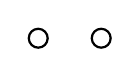
\begin{tikzpicture}[scale=.4]
                \draw[thick] (0cm,0) circle (.3cm);
                \draw[thick] (2cm,0) circle (.3cm);
            \end{tikzpicture} & 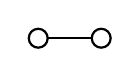
\begin{tikzpicture}[scale=.4]
                \draw[thick] (0cm,0) circle (.3cm);
                \draw[thick] (2cm,0) circle (.3cm);
                \draw[thick] (0.3cm,0) -- +(1.4 cm,0);
            \end{tikzpicture} & 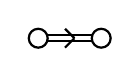
\begin{tikzpicture}[scale=.4]
                \draw[thick] (0cm,0) circle (.3cm);
                \draw[thick] (2cm,0) circle (.3cm);
                \draw[thick] (0.3cm,0.1cm) -- +(1.4 cm,0cm);
                \draw[thick] (0.3cm,-0.1cm) -- +(1.4 cm,0cm);
                \draw[thick] (0.85cm,0.3cm) -- +(0.3cm,-0.3cm);
                \draw[thick] (0.85cm,-0.3cm) -- +(0.3cm,0.3cm);
            \end{tikzpicture} & 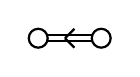
\begin{tikzpicture}[scale=.4]
                \draw[thick] (0cm,0) circle (.3cm);
                \draw[thick] (2cm,0) circle (.3cm);
                \draw[thick] (0.3cm,0.1cm) -- +(1.4 cm,0cm);
                \draw[thick] (0.3cm,-0.1cm) -- +(1.4 cm,0cm);
                \draw[thick] (1.15cm,0.3cm) -- +(-0.3cm,-0.3cm);
                \draw[thick] (1.15cm,-0.3cm) -- +(-0.3cm,0.3cm);
            \end{tikzpicture} & 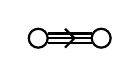
\begin{tikzpicture}[scale=.4]
                \draw[thick] (0cm,0) circle (.3cm);
                \draw[thick] (2cm,0) circle (.3cm);
                \draw[thick] (0.3cm,0.15cm) -- +(1.4 cm,0cm);
                \draw[thick] (0.3cm,0cm) -- +(1.4 cm,0cm);
                \draw[thick] (0.3cm,-0.15cm) -- +(1.4 cm,0cm);
                \draw[thick] (0.85cm,0.3cm) -- +(0.3cm,-0.3cm);
                \draw[thick] (0.85cm,-0.3cm) -- +(0.3cm,0.3cm);
            \end{tikzpicture} & 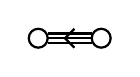
\begin{tikzpicture}[scale=.4]
                \draw[thick] (0cm,0) circle (.3cm);
                \draw[thick] (2cm,0) circle (.3cm);
                \draw[thick] (0.3cm,0.15cm) -- +(1.4 cm,0cm);
                \draw[thick] (0.3cm,0cm) -- +(1.4 cm,0cm);
                \draw[thick] (0.3cm,-0.15cm) -- +(1.4 cm,0cm);
                \draw[thick] (1.15cm,0.3cm) -- +(-0.3cm,-0.3cm);
                \draw[thick] (1.15cm,-0.3cm) -- +(-0.3cm,0.3cm);
            \end{tikzpicture}
    \end{tikzcd} \]
\end{topic}

\begin{example}{dynkin-diagram}
    A complete list of possible Dynkin diagrams is the following: 
    \[ 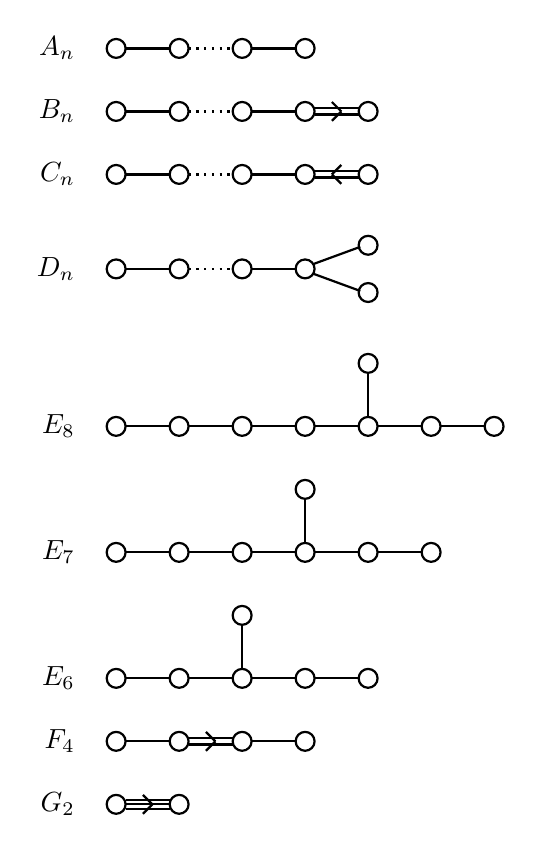
\begin{tikzpicture}[scale=.4]
        % An
        \begin{scope}
            \draw (-1,0) node[anchor=east] {$A_n$};
            \draw[thick] (0cm,0) circle (.3cm);
            \draw[thick] (2cm,0) circle (.3cm);
            \draw[thick] (4cm,0) circle (.3cm);
            \draw[thick] (6cm,0) circle (.3cm);
            \draw[thick] (0.3cm,0) -- +(1.4 cm,0);
            \draw[thick, dotted] (2.3cm,0) -- +(1.4 cm,0);
            \draw[thick] (4.3cm,0) -- +(1.4 cm,0);
        \end{scope}
        % Bn
        \begin{scope}[yshift=-2.0cm]
            \draw (-1,0) node[anchor=east] {$B_n$};
            \draw[thick] (0cm,0) circle (.3cm);
            \draw[thick] (2cm,0) circle (.3cm);
            \draw[thick] (4cm,0) circle (.3cm);
            \draw[thick] (6cm,0) circle (.3cm);
            \draw[thick] (8cm,0) circle (.3cm);
            \draw[thick] (0.3cm,0) -- +(1.4 cm,0);
            \draw[thick, dotted] (2.3cm,0) -- +(1.4 cm,0);
            \draw[thick] (4.3cm,0) -- +(1.4 cm,0);
            \draw[thick] (6.3cm,0.1cm) -- +(1.4 cm,0cm);
            \draw[thick] (6.3cm,-0.1cm) -- +(1.4 cm,0cm);
            \draw[thick] (6.85cm,0.3cm) -- +(0.3cm,-0.3cm);
            \draw[thick] (6.85cm,-0.3cm) -- +(0.3cm,0.3cm);
        \end{scope}
        % Cn
        \begin{scope}[yshift=-4.0cm]
            \draw (-1,0) node[anchor=east] {$C_n$};
            \draw[thick] (0cm,0) circle (.3cm);
            \draw[thick] (2cm,0) circle (.3cm);
            \draw[thick] (4cm,0) circle (.3cm);
            \draw[thick] (6cm,0) circle (.3cm);
            \draw[thick] (8cm,0) circle (.3cm);
            \draw[thick] (0.3cm,0) -- +(1.4 cm,0);
            \draw[thick, dotted] (2.3cm,0) -- +(1.4 cm,0);
            \draw[thick] (4.3cm,0) -- +(1.4 cm,0);
            \draw[thick] (6.3cm,0.1cm) -- +(1.4 cm,0cm);
            \draw[thick] (6.3cm,-0.1cm) -- +(1.4 cm,0cm);
            \draw[thick] (7.15cm,0.3cm) -- +(-0.3cm,-0.3cm);
            \draw[thick] (7.15cm,-0.3cm) -- +(-0.3cm,0.3cm);
        \end{scope}
        % Dn
        \begin{scope}[yshift=-7.0cm]
            \draw (-1,0) node[anchor=east] {$D_n$};
            \draw[thick] (0cm,0) circle (.3cm);
            \draw[thick] (2cm,0) circle (.3cm);
            \draw[thick] (4cm,0) circle (.3cm);
            \draw[thick] (6cm,0) circle (.3cm);
            \draw[thick] (8cm,0.75cm) circle (.3cm);
            \draw[thick] (8cm,-0.75cm) circle (.3cm);
            \draw[thick] (0.3cm,0) -- +(1.4 cm,0);
            \draw[thick, dotted] (2.3cm,0) -- +(1.4 cm,0);
            \draw[thick] (4.3cm,0) -- +(1.4 cm,0);
            \draw[thick] (6.25cm,0.15) -- +(1.5cm,0.55);
            \draw[thick] (6.25cm,-0.15) -- +(1.5cm,-0.55);
        \end{scope}
        % E8
        \begin{scope}[yshift=-12.0cm]
            \draw (-1,0) node[anchor=east] {$E_8$};
            \draw[thick] (0cm,0) circle (.3cm);
            \draw[thick] (2cm,0) circle (.3cm);
            \draw[thick] (4cm,0) circle (.3cm);
            \draw[thick] (6cm,0) circle (.3cm);
            \draw[thick] (8cm,0) circle (.3cm);
            \draw[thick] (10cm,0) circle (.3cm);
            \draw[thick] (12cm,0) circle (.3cm);
            \draw[thick] (8cm,2cm) circle (.3cm);
            \draw[thick] (0.3cm,0) -- +(1.4 cm,0);
            \draw[thick] (2.3cm,0) -- +(1.4 cm,0);
            \draw[thick] (4.3cm,0) -- +(1.4 cm,0);
            \draw[thick] (6.3cm,0) -- +(1.4 cm,0);
            \draw[thick] (8.3cm,0) -- +(1.4 cm,0);
            \draw[thick] (10.3cm,0) -- +(1.4 cm,0);
            \draw[thick] (8cm,0.3cm) -- +(0cm,1.4cm);
        \end{scope}
        % E7
        \begin{scope}[yshift=-16.0cm]
            \draw (-1,0) node[anchor=east] {$E_7$};
            \draw[thick] (0cm,0) circle (.3cm);
            \draw[thick] (2cm,0) circle (.3cm);
            \draw[thick] (4cm,0) circle (.3cm);
            \draw[thick] (6cm,0) circle (.3cm);
            \draw[thick] (8cm,0) circle (.3cm);
            \draw[thick] (10cm,0) circle (.3cm);
            \draw[thick] (6cm,2cm) circle (.3cm);
            \draw[thick] (0.3cm,0) -- +(1.4 cm,0);
            \draw[thick] (2.3cm,0) -- +(1.4 cm,0);
            \draw[thick] (4.3cm,0) -- +(1.4 cm,0);
            \draw[thick] (6.3cm,0) -- +(1.4 cm,0);
            \draw[thick] (8.3cm,0) -- +(1.4 cm,0);
            \draw[thick] (6cm,0.3cm) -- +(0cm,1.4cm);
        \end{scope}
        % E6
        \begin{scope}[yshift=-20.0cm]
            \draw (-1,0) node[anchor=east] {$E_6$};
            \draw[thick] (0cm,0) circle (.3cm);
            \draw[thick] (2cm,0) circle (.3cm);
            \draw[thick] (4cm,0) circle (.3cm);
            \draw[thick] (6cm,0) circle (.3cm);
            \draw[thick] (8cm,0) circle (.3cm);
            \draw[thick] (4cm,2cm) circle (.3cm);
            \draw[thick] (0.3cm,0) -- +(1.4 cm,0);
            \draw[thick] (2.3cm,0) -- +(1.4 cm,0);
            \draw[thick] (4.3cm,0) -- +(1.4 cm,0);
            \draw[thick] (6.3cm,0) -- +(1.4 cm,0);
            \draw[thick] (4cm,0.3cm) -- +(0cm,1.4cm);
        \end{scope}
        % F4
        \begin{scope}[yshift=-22.0cm]
            \draw (-1,0) node[anchor=east] {$F_4$};
            \draw[thick] (0cm,0) circle (.3cm);
            \draw[thick] (2cm,0) circle (.3cm);
            \draw[thick] (4cm,0) circle (.3cm);
            \draw[thick] (6cm,0) circle (.3cm);
            \draw[thick] (0.3cm,0) -- +(1.4 cm,0);
            \draw[thick] (4.3cm,0) -- +(1.4 cm,0);
            \draw[thick] (2.3cm,0.1cm) -- +(1.4 cm,0);
            \draw[thick] (2.3cm,-0.1cm) -- +(1.4 cm,0);
            \draw[thick] (2.85cm,0.3cm) -- +(0.3cm,-0.3cm);
            \draw[thick] (2.85cm,-0.3cm) -- +(0.3cm,0.3cm);
        \end{scope}
        % G2
        \begin{scope}[yshift=-24.0cm]
            \draw (-1,0) node[anchor=east] {$G_2$};
            \draw[thick] (0cm,0) circle (.3cm);
            \draw[thick] (2cm,0) circle (.3cm);
            \draw[thick] (0.3cm,0.15cm) -- +(1.4 cm,0cm);
            \draw[thick] (0.3cm,0cm) -- +(1.4 cm,0cm);
            \draw[thick] (0.3cm,-0.15cm) -- +(1.4 cm,0cm);
            \draw[thick] (0.85cm,0.3cm) -- +(0.3cm,-0.3cm);
            \draw[thick] (0.85cm,-0.3cm) -- +(0.3cm,0.3cm);
        \end{scope}
    \end{tikzpicture} \]
\end{example}

\begin{topic}{lie-algebra-representation}{Lie algebra representation}
    Let $\mathfrak{g}$ be a \tref{lie-algebra}{Lie algebra} over a field $k$. A \textbf{Lie algebra representation} of $\mathfrak{g}$ on a \tref{LA:vector-space}{vector space} $V$ over $k$ is a Lie algebra morphism
    \[ \pi : \mathfrak{g} \to \mathfrak{gl}(V) , \]
    where $\mathfrak{gl}(V)$ denotes the Lie algebra of endomorphisms of $V$. Concretely, $\pi$ is a $k$-linear map such that
    \[ \pi([x, y]) = [\pi(x), \pi(y)] \]
    for all $x, y \in \mathfrak{g}$.
\end{topic}

\begin{example}{lie-algebra-representation}
    For any Lie algebra $\mathfrak{g}$, there is the \tref{DG:adjoint-representation}{adjoint representation}
    \[ \textup{ad}_\mathfrak{g} : \mathfrak{g} \to \mathfrak{gl}(\mathfrak{g}), \quad x \mapsto \textup{ad}_x = [x, -] . \]
    Indeed, this is linear map respects the Lie bracket by the Jacobi identity,
    \[ [[x, y], z] = [x, [y, z]] - [y, [x, z]] . \]
\end{example}

\begin{topic}{verma-module}{Verma module}
    Let $\mathfrak{g}$ be a complex \tref{semisimple-lie-algebra}{semisimple Lie algebra}, with \tref{cartan-subalgebra}{Cartan subalgebra} $\mathfrak{h}$ and \tref{root-system-lie-algebra}{root system} $\Phi$. For a choice of positive roots $\Phi^+$, let $\mathfrak{b} \subset \mathfrak{g}$ be the (Borel) subalgebra generated by $\mathfrak{h}$ and all $\mathfrak{g}_\alpha$ with $\alpha \in \Phi^+$. For any $\lambda \in \mathfrak{h}^*$, the \textbf{Verma module} with highest weight $\lambda$ is the $U(\mathfrak{g})$-module
    \[ V_\lambda = U(\mathfrak{g}) \otimes_{U(\mathfrak{b})} \CC_\lambda , \]
    where $U(\mathfrak{g})$ denotes the \tref{universal-enveloping-algebra}{universal enveloping algebra} of $\mathfrak{g}$, and $\CC_\lambda$ is the one-dimensional $U(\mathfrak{b})$-module, where any $h \in \mathfrak{h}$ acts by $\lambda(h)$ and any $x \in \mathfrak{g}_\alpha$ acts by $0$.
    
    The Verma module $V_\lambda$ has the universal property that for any \tref{lie-algebra-representation}{representation} $\pi : \mathfrak{g} \to \mathfrak{gl}(V)$ generated by a highest weight vector of weight $\lambda$, there is a surjective map $V_\lambda \to V$ of representations.
\end{topic}

\begin{example}{verma-module}
    Consider $\mathfrak{g} = \mathfrak{sl}_2(\CC)$ with the usual basis
    \[ X = \begin{pmatrix} 0 & 1 \\ 0 & 0 \end{pmatrix}, \quad Y = \begin{pmatrix} 0 & 0 \\ -1 & 0 \end{pmatrix} \quad \textup{ and } \quad H = \begin{pmatrix} 1 & 0 \\ 0 & -1 \end{pmatrix} . \]
    For any $\lambda \in \mathfrak{h}^*$ given by $\lambda(H) = m \in \CC$, the corresponding Verma module $V_\lambda$ is spanned by vectors $v_0, v_1, v_2, \ldots$ and satisfies
    \[ Y \cdot v_j = v_{j + 1}, \quad X \cdot v_j = j(m - (j - 1)) v_{j - 1}, \quad H \cdot v_j = (m - 2j) v_j . \]
    In particular, $X \cdot v_0 = 0$ and $H \cdot v_0 = m v_0$, so $v_0$ is a highest weight vector of weight $m$.
\end{example}

\begin{topic}{casimir-element}{Casimir element}
    Let $\mathfrak{g}$ be a \tref{semisimple-lie-algebra}{semisimple Lie algebra}. For any basis $e_1, \ldots, e_n$ of $\mathfrak{g}$ with dual basis $e^1, \ldots, e^n$ with respect to some non-degenerate bilinear form $B : \mathfrak{g} \times \mathfrak{g} \to k$ (commonly the \tref{killing-form}{Killing form}), the \textbf{Casimir element} of $\mathfrak{g}$ is the element
    \[ \Omega = \sum_{i = 1}^{n} e_i e^i \in U(\mathfrak{g}) , \]
    of the \tref{universal-enveloping-algebra}{universal enveloping algebra} of $\mathfrak{g}$. In particular, it lies in the \tref{ring-center}{center} of $U(\mathfrak{g})$.
\end{topic}

\begin{example}{casimir-element}
    Consider $\mathfrak{g} = \mathfrak{sl}_2(\CC)$ with the usual basis
    \[ X = \begin{pmatrix} 0 & 1 \\ 0 & 0 \end{pmatrix}, \quad Y = \begin{pmatrix} 0 & 0 \\ -1 & 0 \end{pmatrix} \quad \textup{ and } \quad H = \begin{pmatrix} 1 & 0 \\ 0 & -1 \end{pmatrix} . \]
    With respect to the Killing form $\kappa_\mathfrak{g}$, we have
    \[ \kappa_\mathfrak{g}(X, X) = 0, \quad \kappa_\mathfrak{g}(X, Y) = 4, \quad \kappa_\mathfrak{g}(X, H) = 0, \]
    \[ \kappa_\mathfrak{g}(Y, Y) = 0, \quad \kappa_\mathfrak{g}(Y, H) = 0, \quad \kappa_\mathfrak{g}(H, H) = 8, \]
    so it follows that $X^* = \frac{1}{4} Y$, $Y^* = \frac{1}{4} X$ and $H^* = \frac{1}{8} H$. Hence, the Casimir element of $\mathfrak{sl}_2(\CC)$ is
    \[ \frac{1}{4} XY + \frac{1}{4} YX + \frac{1}{8} H^2 \in U(\mathfrak{sl}_2(\CC)) . \]
    Since $\Omega$ is central, it acts by a scalar on every representation of $\mathfrak{g}$. In this case, for a representation $V$ of highest weight $m$, the Casimir element $\Omega$ acts by the scalar $\frac{1}{8} m(m + 2)$.
\end{example}

\begin{topic}{manin-triple}{Manin triple}
    A \textbf{Manin triple} $(\mathfrak{g}, \mathfrak{g}^+, \mathfrak{g}^-)$ consists of a \tref{lie-algebra}{Lie algebra} $\mathfrak{g}$ with a non-degenerate invariant symmetric bilinear form $\langle \cdot, \cdot \rangle$ on $\mathfrak{g}$, together with two isotropic \tref{LA:complementary-subspaces}{complementary subspaces} $\mathfrak{g}^+, \mathfrak{g}^- \subset \mathfrak{g}$.
\end{topic}

\begin{topic}{theorem-highest-weight}{theorem of the highest weight}
    Let $\mathfrak{g}$ be a complex \tref{semisimple-lie-algebra}{semisimple Lie algebra}, with \tref{cartan-subalgebra}{Cartan subalgebra} $\mathfrak{h}$, \tref{root-system-lie-algebra}{root system} $\Phi$, and a choice of positive roots $\Phi^+$. An element $\lambda \in \mathfrak{h}^*$ is \textbf{integral} if $2 \frac{(\lambda, \alpha)}{(\alpha, \alpha)}$ is an integer for all $\alpha \in \Phi$, and called \textbf{dominant} if $(\lambda, \alpha) \ge 0$ for all $\alpha \in \Phi^+$. Furthermore, an element $\mu \in \mathfrak{h}^*$ is \textbf{higher} than an element $\lambda \in \mathfrak{h}^*$ if $\mu - \lambda$ can be expressed as a linear combination of positive roots with non-negative real coefficients. Finally, a weight of a representation of $\mathfrak{g}$ is called a \textbf{highest weight} if it is higher than every other weight of of that representation.
    
    The \textbf{theorem of the highest weight} states that
    \begin{enumerate}[(i)]
        \item Every irreducible, finite-dimensional \tref{lie-algebra-representation}{representation} of $\mathfrak{g}$ has a highest weight, which is dominant and integral.
        \item Two irreducible, finite-dimensional representations of $\mathfrak{g}$ with the same highest weight are isomorphic.
        \item For every dominant integral element $\mu \in \mathfrak{h}^*$, there exists an irreducible, finite-dimensional representation of $\mathfrak{g}$ with highest weight $\mu$.
    \end{enumerate}
\end{topic}

\begin{topic}{pbw-theorem}{Poincaré--Birkhoff--Witt theorem}
    Let $\mathfrak{g}$ be a finite-dimensional \tref{lie-algebra}{Lie algebra} with \tref{LA:basis}{basis} $X_1, \ldots, X_n$. The \textbf{Poincaré--Birkhoff--Witt theorem} states that the elements
    \[ X_1^{k_1} X_2^{k_2} \cdots X_n^{k_n}, \qquad \textup{ with } k_i \ge 0 ,  \]
    form a basis of the \tref{universal-enveloping-algebra}{universal enveloping algebra} $U(\mathfrak{g})$.
\end{topic}

\begin{topic}{dg-lie-algebra}{differential graded Lie algebra}
    A \textbf{differential graded Lie algebra (dgla)} over a \tref{field}{field} $k$ is a \tref{HA:chain-complex}{chain complex} $(\mathfrak{g}_\bdot, d)$ of $k$-modules with a bilinear map $[\cdot, \cdot] : \mathfrak{g}_p \otimes \mathfrak{g}_q \to \mathfrak{g}_{p + q}$ satisfying
    \begin{itemize}
        \item (\textit{graded derivation}) $d[x, y] = [dx, y] + (-1)^p [x, dy]$ for all $x \in \mathfrak{g}_p$ and $y \in \mathfrak{g}_q$,
        \item (\textit{graded skew-symmetry}) $[x, y] = -(-1)^{pq} [y, x]$ for all $x \in \mathfrak{g}_p$ and $y \in \mathfrak{g}_q$,
        \item (\textit{graded Jacobi identity}) $[x, [y, z]] = [[x, y], z] + (-1)^{pq} [y, [x, z]]$ for all $x \in \mathfrak{g}_p$, $y \in \mathfrak{g}_q$, and $z \in \mathfrak{g}_r$.
    \end{itemize}
\end{topic}

\begin{example}{dg-lie-algebra}
    Any \tref{dg-algebra}{differential graded algebra} $(A_\bdot, d)$ has the structure of a differential graded Lie algebra with bracket
    \[ [\cdot, \cdot] : A_p \otimes A_q \to A_{p + q}, \quad [x, y] = xy - (-1)^{pq} yx, \quad x \in A_p, y \in A_q . \]
    % This yields a (forgetful) functor $\textbf{Alg}^\textup{dg}_k \to \textbf{Lie}^\textup{dg}_k$, which has a \tref{CT:adjunction}{left adjoint} $U : \textbf{Lie}^\textup{dg}_k \to \textbf{Alg}^\textup{dg}_k$, which assigns to every dgla $\mathfrak{g}_\bdot$ its \textit{universal enveloping algebra} 
    % \[ U(\mathfrak{g}_\bdot) = \bigoplus_{n \ge 0} \mathfrak{g}_\bdot^{\otimes n} / I(\mathfrak{g}_\bdot) , \]
    % where $I(\mathfrak{g}_\bdot)$ is the two-sided ideal generated by all expressions of the form
    % \[ (x \otimes y) - (-1)^{pq} (y \otimes x) - [x, y], \quad x \in \mathfrak{g}_p, y \in \mathfrak{g}_q . \]
\end{example}

\begin{topic}{maurer-cartan-equation}{Maurer--Cartan equation}
    Let $(\mathfrak{g}_\bdot, d, [-, -])$ be a \tref{dg-lie-algebra}{differential graded Lie algebra}. The \textbf{Maurer--Cartan equation} in $\mathfrak{g}_\bdot$ is the equation
    \[ da + \frac{1}{2} [a, a] = 0, \quad a \in \mathfrak{g}_{-1} . \]
    A \textbf{Maurer--Cartan element} of $\mathfrak{g}_\bdot$ is an element $a \in \mathfrak{g}_{-1}$ satisfying the Maurer--Cartan equation.
\end{topic}

\begin{example}{maurer-cartan-equation}
    Let $(V, \partial)$ be a \tref{HA:chain-complex}{chain complex} of $k$-modules, and let $A$ be a \tref{local-ring}{local} \tref{artin-ring}{artin ring} over $k$ with maximal ideal $\mathfrak{m}$. A \textit{deformation} of $V$ over $A$ is a chain complex
    \[ \cdots \xrightarrow{\partial^A_{n + 1}} V_n \otimes_k A \xrightarrow{\partial^A_n} V_{n - 1} \otimes_k A \xrightarrow{\partial^A_{n - 1}} \cdots \]
    which reduces to $(V, \partial)$ modulo $\mathfrak{m}$. The claim is that the deformation theory is controlled by the dgla $\Hom_\bdot(V, V) \otimes_k \mathfrak{m}$, where $\Hom_\bdot(V, V)$ is given by
    \[ \Hom_i(V, V) = \prod_{n \in \ZZ} \Hom(V_n, V_{n + i}) , \]
    with differential and Lie bracket given by
    \[ \begin{aligned}
        d : \Hom_i(V, V) \to \Hom_{i - 1}(V, V), &\qquad df = \partial \circ f - (-1)^{\deg(f)} f \circ \partial , \\
        [ \cdot, \cdot ] : \Hom_i(V, V) \otimes \Hom_j(V, V) \to \Hom_{i + j}(V, V), &\qquad [f, g] = f \circ g - (-1)^{\deg(f) \deg(g)} g \circ f .
    \end{aligned} \]
    Indeed, from the decomposition $A = k \oplus \mathfrak{m}$ as vector spaces, we can write $\partial^A = \partial + \xi$ for some $\xi \in \Hom_{-1}(V, V) \otimes_k \mathfrak{m}$. Now, in order for $(V \otimes_k A, \partial_A)$ to be a chain complex, we must have $(\partial^A)^2 = (\partial + \xi)^2 = \partial^2 + \partial \xi + \xi \partial + \xi^2 = 0$, so
    \[ d \xi + \frac{1}{2} [\xi, \xi] = 0 , \]
    that is, $\xi$ must satisfy the Maurer--Cartan equation.
\end{example}

\begin{example}{maurer-cartan-equation}
    Let $A$ be a commutative $k$-algebra, and consider the notion of a \textit{star product} on $A \llbracket \hbar \rrbracket$, that is, an associative product on $A \llbracket \hbar \rrbracket$ such that $a \star b \equiv ab \mod \hbar$. The claim is that star products are controlled by the \tref{hochschild-homology}{Hochschild cohomology} of $A$.
    
    Let us write $a \star b = ab + \sum_{k \ge 1} \hbar^k C_k(a, b)$, where $C_k$ are bilinear maps. By straightforward rewriting, the associativity condition
    \[ (a \star b) \star c = a \star (b \star c) \]
    in order $k$ is equivalent to
    \[ \partial C_k = \sum_{\substack{r + s = k \\ r, s > 0}} C_r(C_s(a, b), c) - C_r(a, C_s(b, c)) , \]
    for all $a, b, c \in A$.
    
    Now, define a dgla based on the (shifted) Hochschild cohomology
    \[ \mathcal{C} = \bigoplus_{i \ge -1} \mathcal{C}^i, \quad \mathcal{C}^i = \Hom_k(A^{\otimes i + 1}, A) , \]
    with differential $df = (-1)^{i + 1} \partial f$ for $f \in \mathcal{C}^i$ ($\partial$ being the Hochschild-differential), whose product is given by
    \[ (f \circ g)(a_1, \ldots, a_{i + j - 1}) = \sum_{k = 1}^{i} (-1)^{j(k - 1)} f(a_1, \ldots, a_{k - 1}, g(a_k, \ldots, a_{k + j}), \ldots, a_{i + j - 1}) , \] for all $f \in \mathcal{C}^i$ and $g \in \mathcal{C}^j$, and whose bracket is given by the \textit{Gerstenhaber bracket}
    \[ [f, g] = f \circ g - (-1)^{ij} g \circ f \]
    for all $f \in \mathcal{C}^i$ and $g \in \mathcal{C}^j$.
    Then, for any $C = \sum_{k \ge 1} \hbar^k C_k \in \hbar \mathcal{C}^1 \llbracket \hbar \rrbracket$, we obtain
    \[ dC = \sum_{k \ge 1} \hbar \partial C_k \]
    and
    \[ \frac{1}{2} [C, C] = \frac{1}{2} \left[ \sum_{k \ge 0} \hbar C_k, \sum_{k \ge 0} \hbar C_k \right] = \sum_{\substack{r + s = k \\ r, s > 0}} \hbar^k C_r(C_s(a, b), c) - C_r(a, C_s(b, c)) . \]
    Therefore, $C$ is a solution to the Maurer--Cartan equation
    \[ dC + \frac{1}{2}[C, C] = 0 \]
    precisely if $a \star b = ab + \sum_{k \ge 1} \hbar^k C_k(a, b)$ is an associative star product.
\end{example}

\begin{topic}{chevalley-basis}{Chevalley basis}
    Let $\mathfrak{g}$ be a \tref{semisimple-lie-algebra}{semisimple} complex \tref{lie-algebra}{Lie algebra} with \tref{cartan-subalgebra}{Cartan subalgebra} $\mathfrak{h}$ and \tref{root-system-lie-algebra}{root system} $(\mathfrak{h}^*, \Phi)$. For a choice of positive roots, let $\Delta$ be the set of simple roots, and for every simple root $\alpha \in \Delta$, let $H_\alpha \in \mathfrak{h}$ be determined by $\beta(H_\alpha) = 2 \frac{\langle \alpha, \beta \rangle}{\langle \alpha, \alpha \rangle}$ for all $\beta \in \Phi$.
    A \textbf{Chevalley basis} for $\mathfrak{g}$ is a \tref{LA:basis}{basis} of the form $\{ H_\alpha \;:\; \alpha \in \Delta \} \cup \{ X_\alpha \;:\; \alpha \in \Phi \}$ such that
    \begin{itemize}
        \item $[H_\alpha, H_\beta] = 0$ for all $\alpha, \beta \in \Delta$,
        \item $[H_\alpha, X_\beta] = 2 \frac{\langle \beta, \alpha \rangle}{\langle \alpha, \alpha \rangle} X_\beta$ for all $\alpha \in \Delta, \beta \in \Phi$,
        \item $[X_\alpha, X_{-\alpha}] = H_\alpha$ for all $\alpha \in \Phi$,
        \item $[X_\alpha, X_\beta] = \pm (p + 1) X_{\alpha + \beta}$ for all $\alpha, \beta \in \Phi$ such that $\alpha + \beta \in \Phi$, where $p$ is the greatest positive integer such that $\beta - p \alpha$.
    \end{itemize}
    A Chevalley basis always exists.
\end{topic}

\begin{example}{chevalley-basis}
    Consider the Lie algebra $\mathfrak{sl}_2$ with Cartan subalgebra $\mathfrak{h} = \left\{ \left( \begin{smallmatrix} x & 0 \\ 0 & -x \end{smallmatrix} \right) \right\}$ and root system $(\mathfrak{h}^*, \{ \pm \alpha \})$, where $\alpha$ is given by $\alpha \left( \left( \begin{smallmatrix} 1 & 0 \\ 0 & -1 \end{smallmatrix} \right) \right) = 2$. Then a Chevalley basis for $\mathfrak{sl}_2$ is given by
    \[ H_\alpha = \begin{pmatrix} 1 & 0 \\ 0 & -1 \end{pmatrix}, \quad X_\alpha = \begin{pmatrix} 0 & 1 \\ 0 & 0 \end{pmatrix}, \quad X_{-\alpha} = \begin{pmatrix} 0 & 0 \\ 1 & 0 \end{pmatrix} . \]
\end{example}

\begin{topic}{kostant-integral-form}{Kostant integral form}
    Let $\mathfrak{g}$ be a \tref{semisimple-lie-algebra}{semisimple} \tref{lie-algebra}{Lie algebra} over $\CC$, with \tref{chevalley-basis}{Chevalley basis} $\{ H_1, \ldots, H_\ell \} \cup \{ X_\alpha \;:\; \alpha \in \Phi \}$. The \textbf{Kostant $\ZZ$-form} of $\mathfrak{g}$ is the $\ZZ$-subalgebra $U_\ZZ(\mathfrak{g})$ of the \tref{universal-enveloping-algebra}{universal enveloping algebra} $U(\mathfrak{g})$ generated by the elements $X_\alpha^r / r!$ for all $\alpha \in \Phi$ and $r \ge 1$.
\end{topic}

\begin{topic}{chevalley-group}{Chevalley group}
    Let $\mathfrak{g}$ be a \tref{semisimple-lie-algebra}{semisimple} complex \tref{lie-algebra}{Lie algebra}, with \tref{root-system-lie-algebra}{root system} $(\mathfrak{h}^*, \Phi)$, \tref{LA:root-lattice}{root lattice} $Q$ and \tref{LA:weight-lattice}{weight lattice} $P$. For any finite-dimensional faithful \tref{lie-algebra-representation}{representation} $V$ of $\mathfrak{g}$, let $L = L(V) = \ZZ \{ \lambda \in \mathfrak{h}^* \mid V_\lambda \ne 0 \}$ and note that $Q \subset L \subset P$. It can be shown there exists a $\ZZ$-submodule $V_\ZZ \subset V$ which is invariant under the \tref{kostant-integral-form}{Kostant $\ZZ$-form} $U_\ZZ(\mathfrak{g})$. Let $k$ be a field, and write $V_k = V_\ZZ \otimes_\ZZ k$. Now, the \textbf{Chevalley group} $G(\Phi, L, k)$ is the subgroup of $\textup{GL}(V_k)$ generated by all elements
    \[ \exp(t X_\alpha) = 1 + X_\alpha \otimes t + (X_\alpha^2 / 2!) \otimes t^2 + (X_\alpha^3 / 3!) \otimes t^3 + \cdots , \]
    with $\alpha \in \Phi$ and $t \in k$. Note that the infinite sum terminates since $X_\alpha V_\lambda \subset V_{\lambda + \alpha}$ and $V$ is finite-dimensional. It can be shown that the Chevalley group only depends on the root system $\Phi$, the intermediate lattice $Q \subset L \subset P$, and the field $k$.
\end{topic}

% \begin{topic}{hyperalgebra}{hyperalgebra }

% \end{topic}

\begin{topic}{heisenberg-lie-algebra}{Heisenberg Lie algebra}
    Let $V$ be a \tref{LA:vector-space}{vector space} over a \tref{field}{field} $k$, and let $\omega : V \times V \to k$ be a skew-symmetric bilinear form on $V$. The \textbf{Heisenberg Lie algebra} corresponding to $(V, \omega)$ is the \tref{lie-algebra}{Lie algebra} $V \oplus k$ whose Lie bracket is given by
    \[ [ (v, \alpha), (w, \beta) ] = (0, \omega(v, w)) . \]
\end{topic}
